%My project is based on the work done by previous students, who made their master thesis on the same subject but with different data sets obtained from previous field campaigns. In Particular, \cite{jakob} processed the data of the 2015 campaign, that took place from 7 to 22 April 2015, during an episode of anticyclonic conditions. In his work, he had to detect the days in which the instruments measured katabatic winds. For this, he used the past records of the meteorological report to see when there were anticyclonic weather conditions. Also, he analysed the wind profiles and temperature profiles to see if they fitted the description of the katabatic winds. After selecting the days, he computed the Reynolds stress tensor, the sensible heat flux and the turbulent kinetic energy. Is important to highlight that he analysed the region where the maximum of the velocity of the jet is expected to be. As a suggestion for future projects, he points out that it could be interesting to study the turbulence beneath the wind maximum, by placing more sensors in the lower levels of the masts (see section~\ref{instrumentation}).

%Also, my work takes in to account the previous work done by \cite{claudine} and \cite{alban}. Both of them analysed the data from the November 2012 campaign. They followed the same methodology as \citeauthor{jakob} did, analysing the same turbulence characteristics of the jet. The main difference is that their work is focused on adapting the Prandtl analytical model with the different measurements recorded in the field. Another difference is that \citeauthor{claudine} did a spectral analysis of the data. This allowed her to represent the energy as a function of the frequency, with the objective to see the energy cascade characteristic of turbulence. 

\subsection{Objectives}
My objectives for this research project will be to analyse the data from a new mission planned for this the months of January or February, in which there are more sensors installed especially in the bottom and the lower region of the meteorological stations (see section~\ref{instrumentation}). This tackles the limitations found in the previous works mentioned above. 

More specifically, the first step will be to pre-process the data using the EddyPro Software (eddy covariance method). Then, it will be necessary to detect the katabatic wind episodes in the data set, by selecting the data that coincide with the anticyclonic episodes and which temperature and wind profiles coincide with the description of the katabatic winds. After that, I will analyse all the turbulent characteristics of the turbulent jet as \citeauthor{jakob} did. And finally, I will do the spectral analysis of the data as \citeauthor{claudine} did. 

There exist the possibility that the meteorological conditions necessary to do the measurements won't occur during winter or occur after February. In this case, I will analyse the data of 2015 and complete the analyse already done by \citeauthor{jakob}, by doing a spectral analysis of the signals, as \citeauthor{claudine} did with the 2012 data sets.

\subsection{Observational site}

The field campaign is planned to be held in the west face of the Grand Colon mountain, in Belledonne Massif, 10~km East of Grenoble. A topographic map of the area is shown in figure~\ref{fig:obs_site}, where the measuring site is marked with a red cross.

\begin{figure}[!ht]
  \begin{center}
  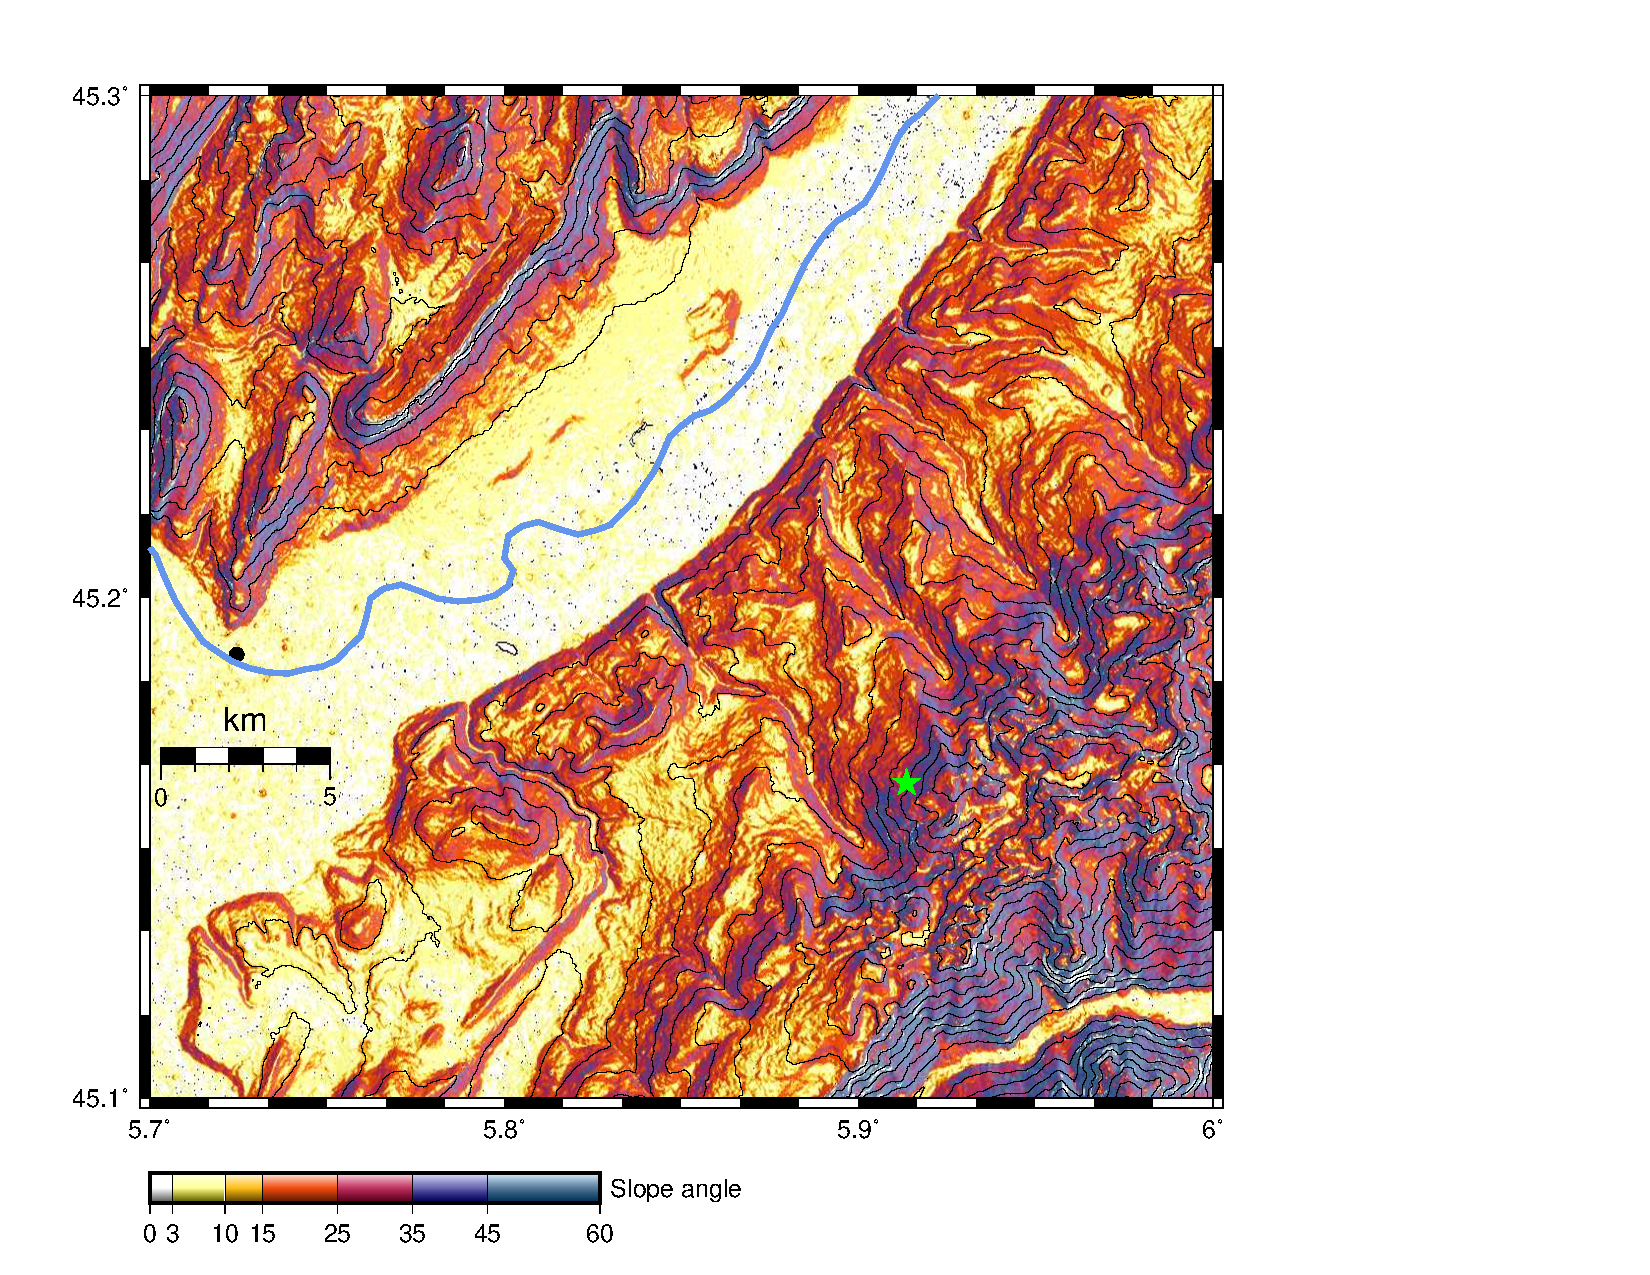
\includegraphics[width=0.8\textwidth]{fig/chapter_1/grenoble_slopes_C100.png}
  \caption{}
  \label{fig:obs_site}
  \end{center}
\end{figure}

The slope in the observational site is around $21\degree$. The meteorological station is going to be located at an altitude of 1770 metres above sea level~\citep{claudine}. All the characterisation of the topography has been done by \cite{alban}.

\subsection{Instrumentation} \label{instrumentation}
The instruments for the next field campaign will be assembled into two masts, which will be located side by side. The mast has been reconfigured to tackle some of the problems and limitations from previous campaigns. We distinguish them by their height, one is 6~m high and the other is 12~m high\footnote{The configuration was altered recently, but couldn't get the most recent schematics. These will certainly change for the presentation.}. 

In figure~\ref{fig:mast_6} we can see the mast that is 6~m high. In it, there are 6 CSAT3 3-D Sonic Anemometers, positioned from 0.4~m to 3.6~m height. These are fixed parallel to the ground. These instruments measure the direction and speed of wind in its three components with a high frequency (around 20~Hz). Currently, Aravind Anandan is doing his research project on the calibration of this instruments and part of his work is calibrating them for this winter mission.

\begin{figure}[!ht]
  \begin{center}
  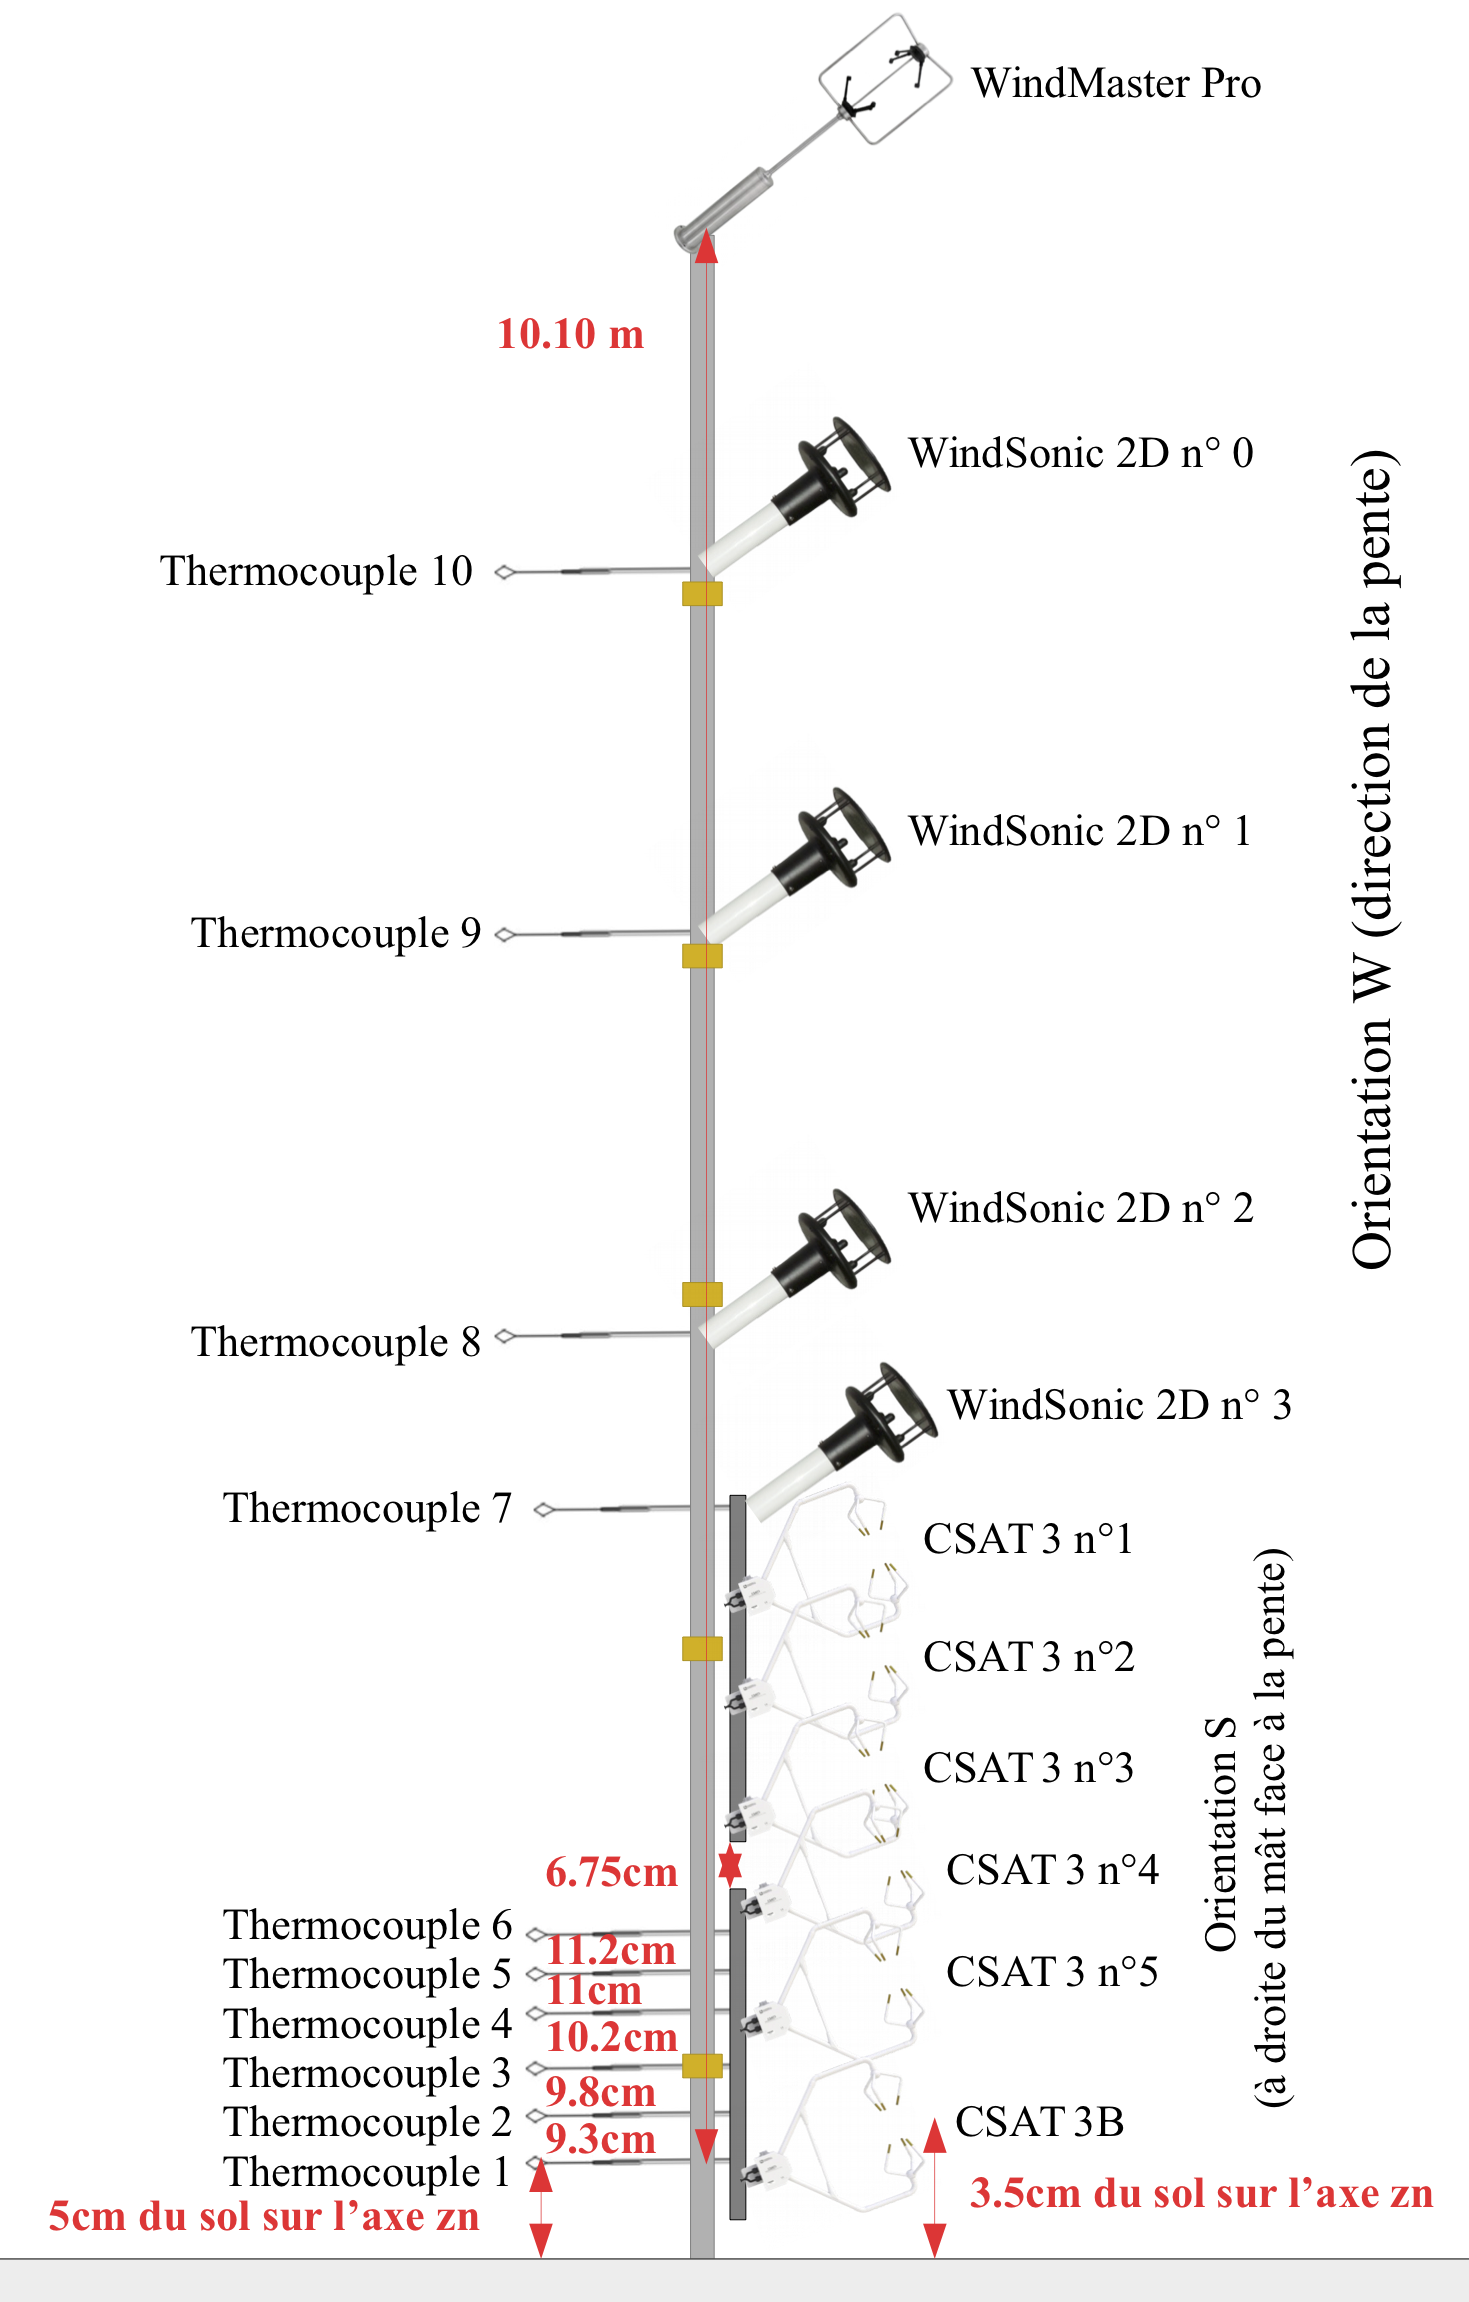
\includegraphics[width=0.7\textwidth]{fig/chapter_1/Montage_J1.png}
  \caption{Placement of the instruments on the 6~m mast. Along the mast, there are six CSAT3 Sonic Anemometers.}
  \label{fig:mast_6}
  \end{center}
\end{figure}

In figure.. we see the mast that is 12~m high. At the top we can see a Windmaster 3D ultrasonic anemometer, that can measure the three components of wind with a frequency up to 20~Hz. Bellow it, we can see three Gill Windmaster anemometers, that are located between 9.5~m and 5.5~m. And at 4.2~m, there is a Vaisala 2D anemometer.  All the anemometers measure the direction and speed of wind with a frequency that depends on the model of the sensor. 

Spread along the mast, there are nine thin film thermocouples, that are used to measure the temperature of air with minimal intrusion. In the middle, there is a radiometer used to measure the radiant flux. Finally, there is an ultrasonic instrument installed in the station (not shown in the figures) to record the height of the snow cover. Snow-covered ground is expected in the measuring site. This is important because the snow decreases the height between the ground and the instruments, which is an important parameter in the calculations.

\section{Timetable}
The timetable~\ref{table:schedule} shows the planning for the activities to do during the next five months. 

\begin{table}[ht!]
%\centering
\begin{center}
\begin{tabular}{|c|c|p{9.5cm}|}
\hline
  & \textbf{Working days} & \textbf{Activity} \\
\hline
January & 1 & Field Work\footnote{\label{note1}The date of the field campaign is not set. It must occur during winter (January and February), when there are anticyclonic conditions.}. Working on theory and foundations of the research.\\
\hline
February & 7 & Field Work$^2$. Analysis of the data, start to analyse 2015 data to get familiar with EddyPro.\\
\hline
March & 4 & Analysis of the data gathered during the field work.\\
\hline
April & 7 & Writing and analysing the data gathered.\\
\hline
May & 12 & Plotting the results and final analysis of the data sets. Working in the final report and oral presentation.\\
\hline
\end{tabular}
\caption{Research project schedule showing the number of working days per month and the tasks to work on.}
\label{table:schedule}
\end{center}
\end{table}